\documentclass[nofonts,nobib]{tufte-handout}

%% Font Stuff
\usepackage{fontspec}
\usepackage{ifxetex}
% \fontspec{EB Garamond}
\setmainfont[Mapping=tex-text,Numbers=OldStyle]{EB Garamond}
\setsansfont{Noto Sans Symbols}
\setmonofont{EB Garamond}
\usepackage{booktabs}
\usepackage{lipsum}

\ifxetex
  \newcommand{\textls}[2][5]{%
    \begingroup\addfontfeatures{LetterSpace=#1}#2\endgroup
  }
  \renewcommand{\allcapsspacing}[1]{\textls[15]{#1}}
  \renewcommand{\smallcapsspacing}[1]{\textls[10]{#1}}
  \renewcommand{\allcaps}[1]{\textls[15]{\MakeTextUppercase{#1}}}
  \renewcommand{\smallcaps}[1]{\smallcapsspacing{\scshape\MakeTextLowercase{#1}}}
  \renewcommand{\textsc}[1]{\smallcapsspacing{\textsmallcaps{#1}}}
\fi

\usepackage[]{biblatex-chicago}
\addbibresource{bibliography.bib}
% % % \DefineBibliographyStrings{english}{%
% %   references = {Works Cited},
% % }


\title{Watch the Tiger Walk: Another Study in Intention}
\author{Rachael Carlson}
\date{\today}
\begin{document}
\maketitle

\section{Introduction}
\newthought{The twenty-first century musician} is faced with a mysterious quagmire. The future of the existence of the professional musician is uncertain. The consumption of music seems to be at all-time highs and yet previous sources of income are unreliable.\sidenote{I don't have a source for this. It would be great to find one.} The musician is no longer able to rely on income from album sales, radio play and other royalties, sheet music sales, or patronage. The twenty-first century musicians appears to require all of these sources in order to make a living as a professional musician. In addition to these sources of income, the musician will need to find income from performances, instruction, YouTube and other internet streaming services royalties, and commissions for publications to magazines. \\

The finger-style guitarist is not immune to these changes. In some cases, the finger-style guitarist was at the forefront of these changes, a harbinger of the times-to-come. One of the earliest YouTube celebrities was Andy McKee. This article will attempt to discern how musicians are surviving, or even thriving, by examining their apparent revenue streams. This article will have two goals. First, to examine the available methods of consuming a twenty-first century musician's output. The aim for this examination is to establish a baseline by which one can measure her progress in relation to those who have achieved notoriety before her. The focus of this research will be on finger-style guitarists primarily.  Second, to examine ``Watch the Tiger Walk'' by Rachael Carlson as a case study in which the means examined in the first portion are fully or partially enacted for a single composition. This may mean several things. I will begin the necessary work on a transcription, I will produce audio and video, I may begin work on reinforcing my website in preparation for a life as a professional musician and finger-style guitarist.

A sign of a healthy musician appears to be her internet presence, calculated by \emph{YouTube} ``views'' and \emph{Facebook} ``likes.''

\section{Internet Presence}
\label{sec:internet-presence}
\newthought{There are numerous} ways in which a twenty-first century musician
supports herself. The most visible component of this support is the
internet. A musician is judged upon her social presence on the internet. 

\subsection{The Data}
\label{sec:data}
The parameters for the research are as follows: finger-style guitarist, a
website, some level of notoriety. I also gave consideration to whether the
artist is established or up-and-coming, ultimately deciding on half
established and half up-and-coming. 42 artist websites were analyzed. 21 artists could be considered up-and-coming and 21 could be
considered established. The original intention was to include artists outside of the finger-style
sphere, however, the data set quickly became too immense. It was necessary to
exclude artists outside of finger-style guitar. It may be beneficial in the
future to take a more inclusive approach to the research in order to inform
the twenty-first century finger-style guitarist. A concerted effort was
made to include musicians outside of the United States. There appears to be a
tendency among burgeoning artists to rely on \emph{Facebook} to share their
craft.

Through an analysis of a subsample of the data, 26 codes were developed. The
codes were carefully selected to demonstrate important elements of an artist's
website. The codes fell into roughly four categories: persona, display,
technologies, and commerce. These codes range from the manner in which the
artist attested to his or her legitimacy to the type of Content Management System (\textsc{cms}) that the artist uses.

This data is a snapshot of the immense world of finger-style guitar as it
exists on the internet. The rapid changes in technology may deem this essay
obsolete in five years. This data set has been included in the appendix.
%   \begin{table*}\centering
%     \small
%     \begin{tabular}{l l}\toprule
%       Artist  &  \\\midrule
%       Title & \emph{Garamond Premier Pro} Display Italic 28pt\\
%       Tuning & \emph{EB Garamond} 12 Regular 10pt\\
%       Octave Designation & \emph{EB Garamond} 12 Regular 10pt subscript\\
%       Composer & \emph{EB Garamond} 12 Regular 10pt\\
%       Clef & \emph{Adobe Garamond Pro} Bold 11pt\\
%       Noteheads & \emph{Noto Sans} Regular 12pt\\
%       Left-Hand Fingering & \emph{Noto Sans} Symbols 12pt\\
%       Right-Hand Fingering & \emph{EB Garamond} 08 Regular 8pt\\
%       Copyright and Page Numbers & \emph{EB Garamond} 08 Regular 8pt\\
%       \bottomrule
%   \end{tabular}
%     \caption{DESCRIBE THE DATA IN AN INTELLIGENT MANNER. Each artist's website is listed in the References section.}
% \end{table*}
\subsection{The Analysis}
\label{sec:analysis}



\section{Transcription}
\newthought{A distinguishing characteristic} of the finger-style guitarist's website is a section of sheet music, scores, or transcriptions of the artist's works. This seems to be a unique component of the finger-style culture. Sadly, while the transcriptions are becoming marginally better than ANSI-Tab on the internet, the quality of the transcriptions produced by these musicians is not on par with the quality of playing or composition. This could be attributed to different factors, all of which are for another essay.
\subsection{Methods}
\label{sec:methods}
The primary method espoused by the University of Wisconsin-Milwaukee (\textsc{uwm}) and Stropes Editions, Ltd. (\textsc{sel}) is a double-impression method utilizing Finale and Adobe InDesign. The methods in this document are as follows: {\XeLaTeX} for the typesetting of this essay and the same double-impression method of Finale and Adobe InDesign used by \textsc{sel} and \textsc{uwm}.

\subsection{Typography}
\label{sec:typography}
The fonts used at \textsc{sel} are Helvetica LT Std and ITC Franklin Gothic. Due to the innovations in finger-style guitar typesetting by this company, it can be difficult to reach beyond the conventions established. I am reminded of a quote by the highly influential designer, Paul Rand, ``new becomes threatening, the old reassuring.''\footnote[][-60pt]{I need to find a citation for this. It might be in Paul Rand, \emph{Paul Rand: A Designer's Art}, (New Haven: Yale University Press, 1985) or Paul Rand, \emph{From Lascaux to Brooklyn}, (New Haven: Yale University Press, 1985), or Paul Rand, \emph{Design Form and Chaos}, (New Haven: Yale University Press, 1993).}
\begin{figure*}\centering
        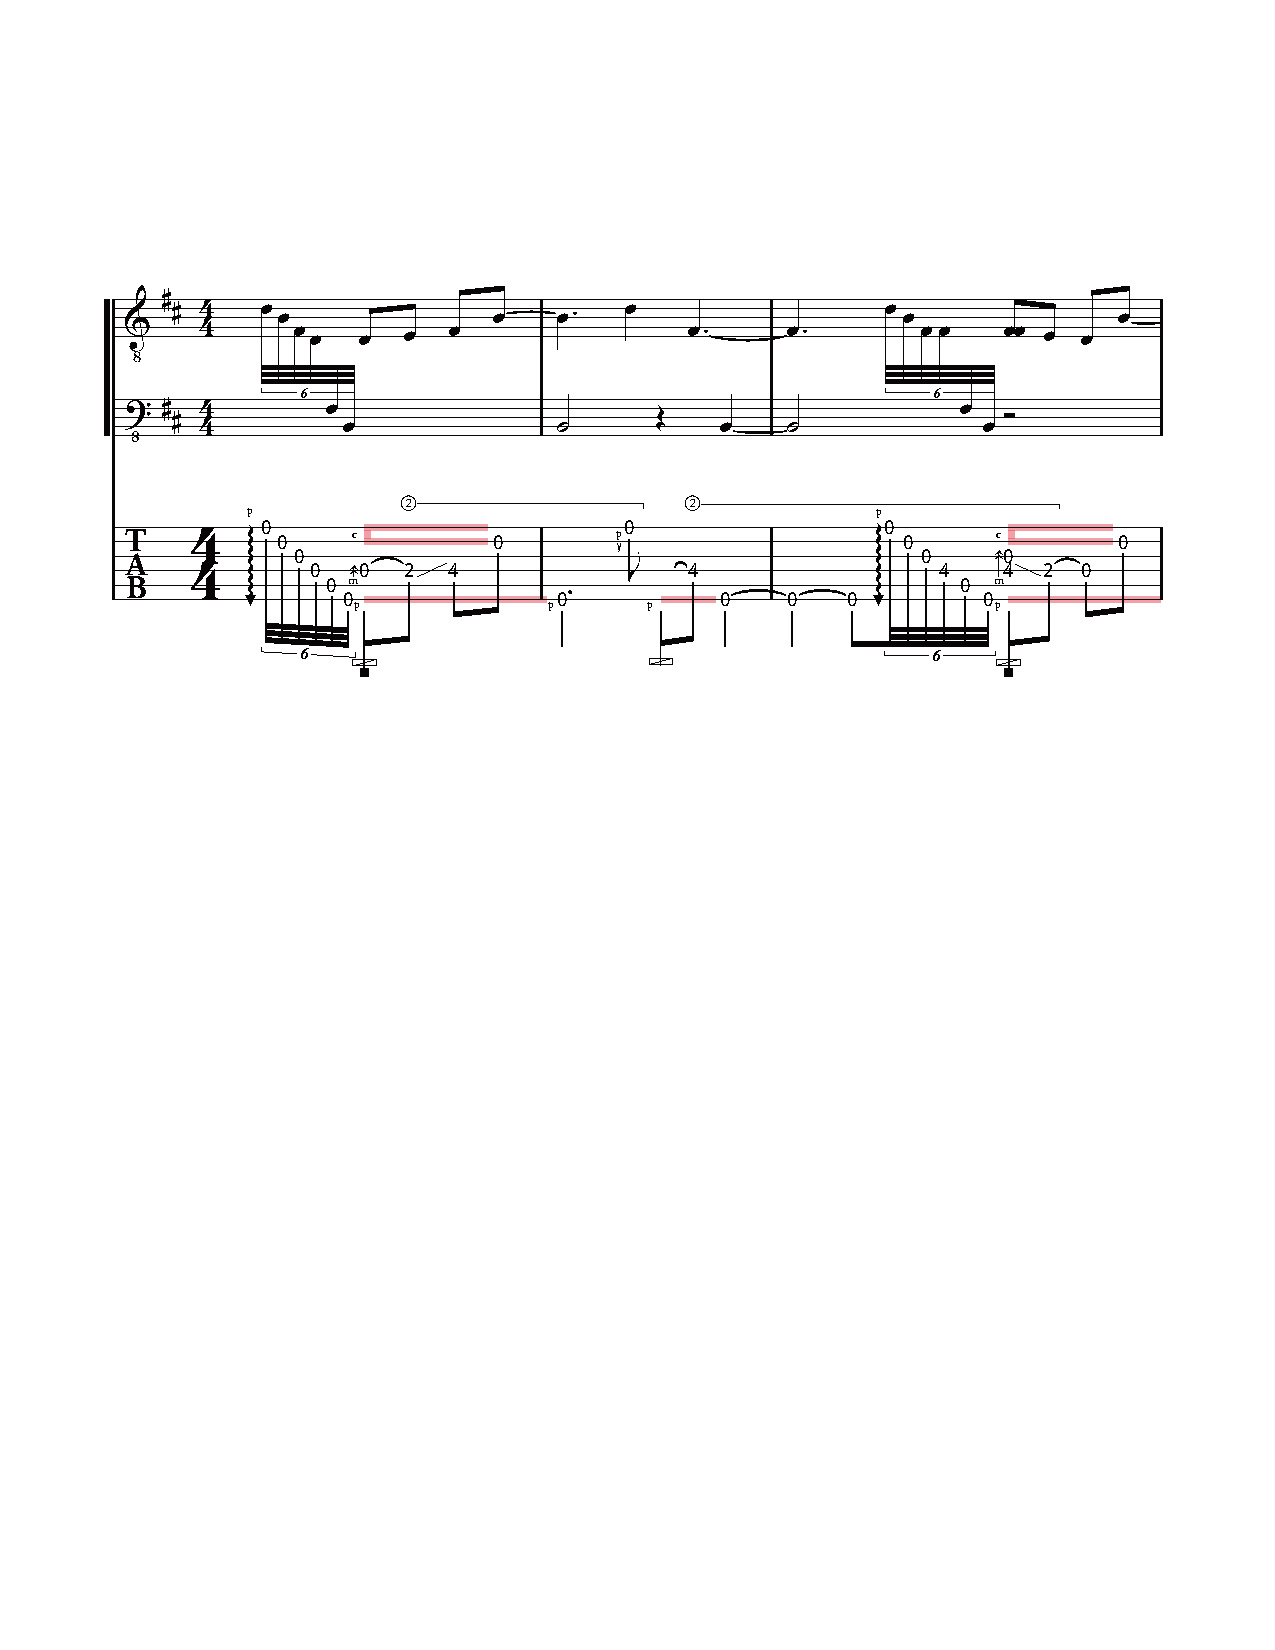
\includegraphics[width=1.00\textwidth]{watchTheTigerWalk1-2c.pdf}
    \caption{``Watch the Tiger Walk'' by Rachael Carlson, mm. 1--2.}
    \label{fig:somthing}
  \end{figure*}
  While the design of the \textsc{sel} sheet music would not be considered bad, in fact they stand apart from all previous transcriptions in their beauty, they \emph{have} established themselves as reassuring. It can be quite difficult to produce a score for finger-style guitar which does not either copy \textsc{sel} or fall into the category of ugly music for the guitar. The difficulty of producing a unique voice within the field of music engraving is perhaps due to this feeling of reassurance. We are tasked with the necessity of simultaneously producing documents that are almost audible in their beauty and ensuring the maximum level of legibility. Established music publishers such as Bärenreiter and Henle Verlag may have specific guidelines to produce a base-level of legibility. Perhaps, the requirement of legibility at a specific distance from the page in order to anticipate real-world scenario of music reading.


  I have carefully chosen the typography of my transcriptions. And while I wish that I could say that I have found the perfect combination, I can not. What I can say, is that the typography that I have chosen for my transcriptions is designed for optimal legibility at small font sizes while ensuring the reader will not confuse one glyph for another.
  \begin{table}\centering
    \small
    \begin{tabular}{l l}\toprule
      Page Content  & Font \\\midrule
      Title & \emph{Garamond Premier Pro} Display Italic 28pt\\
      Tuning & \emph{EB Garamond} 12 Regular 10pt\\
      Octave Designation & \emph{EB Garamond} 12 Regular 10pt subscript\\
      Composer & \emph{EB Garamond} 12 Regular 10pt\\
      Clef & \emph{Adobe Garamond Pro} Bold 11pt\\
      Noteheads & \emph{Noto Sans} Regular 12pt\\
      Left-Hand Fingering & \emph{Noto Sans} Symbols 12pt\\
      Right-Hand Fingering & \emph{EB Garamond} 08 Regular 8pt\\
      Copyright and Page Numbers & \emph{EB Garamond} 08 Regular 8pt\\
      \bottomrule
  \end{tabular}
    \caption{Weights and sizes of fonts used in my transcriptions.}
\end{table}
Fonts that are designed based upon Claude Garamont (c. 1510 -- 1561) and Robert Granjon (1513 -- 1590) speak to me. Both Garamont and Granjon were French type designers and publishers in France. EB Garamond is an open source project directed by Georg Duffner based upon the \emph{Berner specimen}. This specimen does not contain bold examples. As such, neither does EB Garamond. The default numerical figures used in EB Garamond are old-style. Due to this I use Adobe Garamond Pro for titling which contains numbers and for the clef which looks more attractive in a bold typeface. On the complete opposite end of the Garamond spectrum, for the noteheads and the left-hand fingering I use Google's Noto Sans. This font family was designed for the mobile market as a means to ensure that almost all of the more than 128,000 figures in \emph{The Unicode Standard} are present such than when a user is confronted with a glyph they do not see a white box affectionately called a block of tofu. 

There must to be a time when one makes a decision knowing all of the positives and negatives associated with that decision. It is at this point that it is more important that one makes \emph{a} decision than whether that decision is the best possible decision. I have vacillated between ten or so different fonts for my transcriptions. The decision of which font combination ensures readability while expressing an individual voice. This is an extremely difficult set of decisions. If I had enough money to purchase fonts I would most likely use \emph{Garamond Premier Pro} from Adobe and \emph{Whitney} from Hoefler \& Company.\autocites{garamondPremier,hoeflerWhitney} I am attracted to \emph{Whitney} in particular due to the presence of the ``Index'' font subset which contains circled numbers and letters --- \textsf{① ② ③ ④ Ⓣ}. \emph{Garamond Premier Pro} is a massive font family of 34 different fonts each with a different purpose.


% \bibliographystyle{chicagoa}
% \bibliography{bibliography}
\printbibliography
\end{document}
%%% Local Variables:
%%% mode: latex
%%% TeX-master: t
%%% End:
